\documentclass{standalone}
\usepackage{tikz}
\usetikzlibrary{patterns, positioning}


\begin{document}
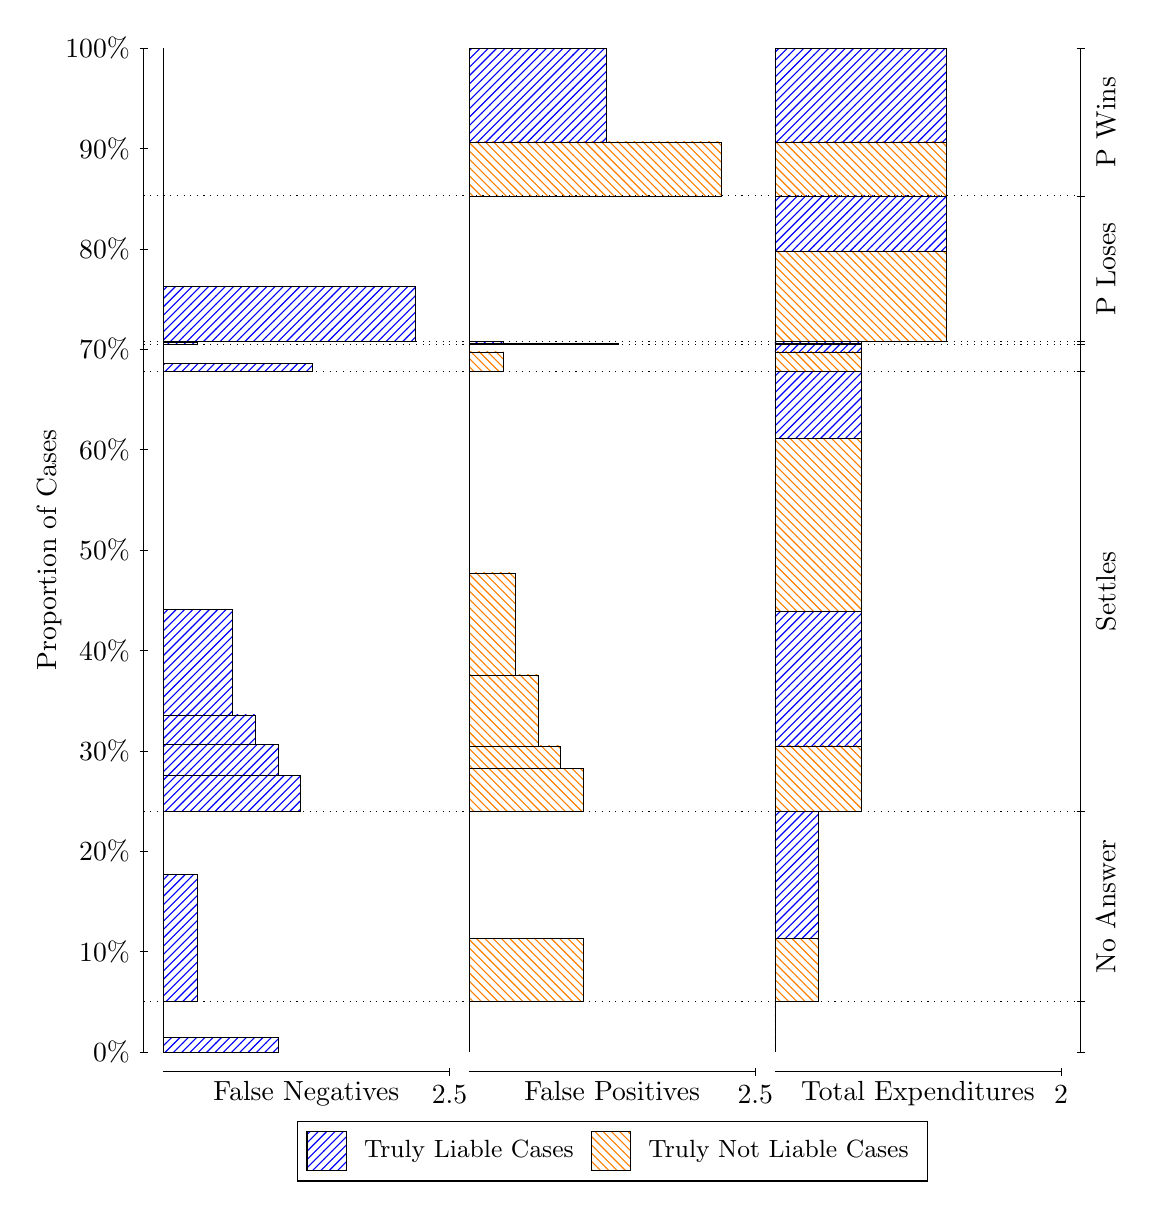
\begin{tikzpicture}
\draw[black, very thin] (1.5,1.75) -- (1.5,14.5);
\node[rotate=90, text=black, anchor=center] at (0.3, 8.125) {Proportion of Cases};
\draw[black, very thin] (1.45,1.75) -- (1.55,1.75);
\node[text=black, anchor=east] at (1.45, 1.75) {0\%};
\draw[black, very thin] (1.45,3.025) -- (1.55,3.025);
\node[text=black, anchor=east] at (1.45, 3.025) {10\%};
\draw[black, very thin] (1.45,4.3) -- (1.55,4.3);
\node[text=black, anchor=east] at (1.45, 4.3) {20\%};
\draw[black, very thin] (1.45,5.575) -- (1.55,5.575);
\node[text=black, anchor=east] at (1.45, 5.575) {30\%};
\draw[black, very thin] (1.45,6.85) -- (1.55,6.85);
\node[text=black, anchor=east] at (1.45, 6.85) {40\%};
\draw[black, very thin] (1.45,8.125) -- (1.55,8.125);
\node[text=black, anchor=east] at (1.45, 8.125) {50\%};
\draw[black, very thin] (1.45,9.4) -- (1.55,9.4);
\node[text=black, anchor=east] at (1.45, 9.4) {60\%};
\draw[black, very thin] (1.45,10.675) -- (1.55,10.675);
\node[text=black, anchor=east] at (1.45, 10.675) {70\%};
\draw[black, very thin] (1.45,11.95) -- (1.55,11.95);
\node[text=black, anchor=east] at (1.45, 11.95) {80\%};
\draw[black, very thin] (1.45,13.225) -- (1.55,13.225);
\node[text=black, anchor=east] at (1.45, 13.225) {90\%};
\draw[black, very thin] (1.45,14.5) -- (1.55,14.5);
\node[text=black, anchor=east] at (1.45, 14.5) {100\%};

\draw[black, very thin] (13.4,1.75) -- (13.4,14.5);
\draw[black, very thin] (13.35,1.75) -- (13.45,1.75);
\node[anchor=west] at (13.35, 1.75) {};
\draw[black, very thin] (13.35,2.3918) -- (13.45,2.3918);
\node[anchor=west] at (13.35, 2.3918) {};
\draw[black, very thin] (13.35,4.8056) -- (13.45,4.8056);
\node[anchor=west] at (13.35, 4.8056) {};
\draw[black, very thin] (13.35,10.397) -- (13.45,10.397);
\node[anchor=west] at (13.35, 10.397) {};
\draw[black, very thin] (13.35,10.736) -- (13.45,10.736);
\node[anchor=west] at (13.35, 10.736) {};
\draw[black, very thin] (13.35,10.772) -- (13.45,10.772);
\node[anchor=west] at (13.35, 10.772) {};
\draw[black, very thin] (13.35,12.622) -- (13.45,12.622);
\node[anchor=west] at (13.35, 12.622) {};
\draw[black, very thin] (13.35,14.5) -- (13.45,14.5);
\node[anchor=west] at (13.35, 14.5) {};

\draw[black, very thin, pattern color=blue, pattern=north east lines] (1.75,1.75) rectangle (3.2033,1.9349);
\draw[black, very thin, pattern color=orange, pattern=north west lines] (1.75,1.9349) rectangle (1.75,2.3918);
\draw[black, very thin, pattern color=blue, pattern=north east lines] (1.75,2.3918) rectangle (2.186,4.0086);
\draw[black, very thin, pattern color=orange, pattern=north west lines] (1.75,4.0086) rectangle (1.75,4.8056);
\draw[black, very thin, pattern color=blue, pattern=north east lines] (1.75,4.8056) rectangle (3.494,5.2625);
\draw[black, very thin, pattern color=blue, pattern=north east lines] (1.75,5.2625) rectangle (3.2033,5.6589);
\draw[black, very thin, pattern color=blue, pattern=north east lines] (1.75,5.6589) rectangle (2.9127,6.0311);
\draw[black, very thin, pattern color=blue, pattern=north east lines] (1.75,6.0311) rectangle (2.622,7.3681);
\draw[black, very thin, pattern color=orange, pattern=north west lines] (1.75,7.3681) rectangle (1.75,10.397);
\draw[black, very thin, pattern color=blue, pattern=north east lines] (1.75,10.397) rectangle (3.6393,10.492);
\draw[black, very thin, pattern color=orange, pattern=north west lines] (1.75,10.492) rectangle (1.75,10.736);
\draw[black, very thin, pattern color=blue, pattern=north east lines] (1.75,10.736) rectangle (2.186,10.761);
\draw[black, very thin, pattern color=orange, pattern=north west lines] (1.75,10.761) rectangle (1.75,10.772);
\draw[black, very thin, pattern color=blue, pattern=north east lines] (1.75,10.772) rectangle (4.9473,11.47);
\draw[black, very thin, pattern color=orange, pattern=north west lines] (1.75,11.47) rectangle (1.75,12.622);
\draw[black, very thin, pattern color=orange, pattern=north west lines] (1.75,12.622) rectangle (1.75,13.307);
\draw[black, very thin, pattern color=blue, pattern=north east lines] (1.75,13.307) rectangle (1.75,14.5);
\draw[black, very thin, pattern color=orange, pattern=north west lines] (5.6333,1.75) rectangle (5.6333,2.2069);
\draw[black, very thin, pattern color=blue, pattern=north east lines] (5.6333,2.2069) rectangle (5.6333,2.3918);
\draw[black, very thin, pattern color=orange, pattern=north west lines] (5.6333,2.3918) rectangle (7.0867,3.1888);
\draw[black, very thin, pattern color=blue, pattern=north east lines] (5.6333,3.1888) rectangle (5.6333,4.8056);
\draw[black, very thin, pattern color=orange, pattern=north west lines] (5.6333,4.8056) rectangle (7.0867,5.354);
\draw[black, very thin, pattern color=orange, pattern=north west lines] (5.6333,5.354) rectangle (6.796,5.6371);
\draw[black, very thin, pattern color=orange, pattern=north west lines] (5.6333,5.6371) rectangle (6.5053,6.5391);
\draw[black, very thin, pattern color=orange, pattern=north west lines] (5.6333,6.5391) rectangle (6.2147,7.8348);
\draw[black, very thin, pattern color=blue, pattern=north east lines] (5.6333,7.8348) rectangle (5.6333,10.397);
\draw[black, very thin, pattern color=orange, pattern=north west lines] (5.6333,10.397) rectangle (6.0693,10.641);
\draw[black, very thin, pattern color=blue, pattern=north east lines] (5.6333,10.641) rectangle (5.6333,10.736);
\draw[black, very thin, pattern color=orange, pattern=north west lines] (5.6333,10.736) rectangle (7.5227,10.746);
\draw[black, very thin, pattern color=blue, pattern=north east lines] (5.6333,10.746) rectangle (6.0693,10.772);
\draw[black, very thin, pattern color=orange, pattern=north west lines] (5.6333,10.772) rectangle (5.6333,11.924);
\draw[black, very thin, pattern color=blue, pattern=north east lines] (5.6333,11.924) rectangle (5.6333,12.622);
\draw[black, very thin, pattern color=orange, pattern=north west lines] (5.6333,12.622) rectangle (8.8307,13.307);
\draw[black, very thin, pattern color=blue, pattern=north east lines] (5.6333,13.307) rectangle (7.3773,14.5);
\draw[black, very thin, pattern color=orange, pattern=north west lines] (9.5167,1.75) rectangle (9.5167,2.2069);
\draw[black, very thin, pattern color=blue, pattern=north east lines] (9.5167,2.2069) rectangle (9.5167,2.3918);
\draw[black, very thin, pattern color=orange, pattern=north west lines] (9.5167,2.3918) rectangle (10.062,3.1888);
\draw[black, very thin, pattern color=blue, pattern=north east lines] (9.5167,3.1888) rectangle (10.062,4.8056);
\draw[black, very thin, pattern color=orange, pattern=north west lines] (9.5167,4.8056) rectangle (10.607,5.6371);
\draw[black, very thin, pattern color=blue, pattern=north east lines] (9.5167,5.6371) rectangle (10.607,7.3463);
\draw[black, very thin, pattern color=orange, pattern=north west lines] (9.5167,7.3463) rectangle (10.607,9.544);
\draw[black, very thin, pattern color=blue, pattern=north east lines] (9.5167,9.544) rectangle (10.607,10.397);
\draw[black, very thin, pattern color=orange, pattern=north west lines] (9.5167,10.397) rectangle (10.607,10.641);
\draw[black, very thin, pattern color=blue, pattern=north east lines] (9.5167,10.641) rectangle (10.607,10.736);
\draw[black, very thin, pattern color=orange, pattern=north west lines] (9.5167,10.736) rectangle (10.607,10.746);
\draw[black, very thin, pattern color=blue, pattern=north east lines] (9.5167,10.746) rectangle (10.607,10.772);
\draw[black, very thin, pattern color=orange, pattern=north west lines] (9.5167,10.772) rectangle (11.697,11.924);
\draw[black, very thin, pattern color=blue, pattern=north east lines] (9.5167,11.924) rectangle (11.697,12.622);
\draw[black, very thin, pattern color=orange, pattern=north west lines] (9.5167,12.622) rectangle (11.697,13.307);
\draw[black, very thin, pattern color=blue, pattern=north east lines] (9.5167,13.307) rectangle (11.697,14.5);
\draw[black, dotted] (1.5,2.3918) -- (13.4,2.3918);
\draw[black, dotted] (1.5,4.8056) -- (13.4,4.8056);
\draw[black, dotted] (1.5,10.397) -- (13.4,10.397);
\draw[black, dotted] (1.5,10.736) -- (13.4,10.736);
\draw[black, dotted] (1.5,10.772) -- (13.4,10.772);
\draw[black, dotted] (1.5,12.622) -- (13.4,12.622);
\draw[black, very thin] (1.75,1.5) -- (5.3833,1.5);
\node[text=black, anchor=north] at (3.5667, 1.5) {False Negatives};
\draw[black, very thin] (5.3833,1.45) -- (5.3833,1.55);
\node[text=black, anchor=north] at (5.3833, 1.45) {2.5};

\draw[black, very thin] (5.6333,1.5) -- (9.2667,1.5);
\node[text=black, anchor=north] at (7.45, 1.5) {False Positives};
\draw[black, very thin] (9.2667,1.45) -- (9.2667,1.55);
\node[text=black, anchor=north] at (9.2667, 1.45) {2.5};

\draw[black, very thin] (9.5167,1.5) -- (13.15,1.5);
\node[text=black, anchor=north] at (11.333, 1.5) {Total Expenditures};
\draw[black, very thin] (13.15,1.45) -- (13.15,1.55);
\node[text=black, anchor=north] at (13.15, 1.45) {2};


\node[text=black, centered, rotate=90] at (13.72, 3.5987) {No Answer};
\node[text=black, centered, rotate=90] at (13.72, 7.6014) {Settles};


\node[text=black, centered, rotate=90] at (13.72, 11.697) {P Loses};
\node[text=black, centered, rotate=90] at (13.72, 13.561) {P Wins};

\draw (7.449999999999999,1.5) node[draw=none] (baseCoordinate) {};
\begin{scope}[align=center]
        \matrix[scale=0.5, draw=black, below=0.5cm of baseCoordinate, nodes={draw}, column sep=0.1cm]{
            \node[rectangle, draw, minimum width=0.5cm, minimum height=0.5cm, pattern color=blue, pattern=north east lines] {}; &
            \node[draw=none, font=\small, text=black] (B) {Truly Liable Cases}; &
            \node[rectangle, draw, minimum width=0.5cm, minimum height=0.5cm, pattern color=orange, pattern=north west lines] {}; &
            \node[draw=none, font=\small, text=black] (B) {Truly Not Liable Cases}; \\
            };
\end{scope}

\end{tikzpicture}
\end{document}